% Options for packages loaded elsewhere
\PassOptionsToPackage{unicode}{hyperref}
\PassOptionsToPackage{hyphens}{url}
%
\documentclass[
  english,
  man,man,floatsintext]{apa6}
\usepackage{lmodern}
\usepackage{amssymb,amsmath}
\usepackage{ifxetex,ifluatex}
\ifnum 0\ifxetex 1\fi\ifluatex 1\fi=0 % if pdftex
  \usepackage[T1]{fontenc}
  \usepackage[utf8]{inputenc}
  \usepackage{textcomp} % provide euro and other symbols
\else % if luatex or xetex
  \usepackage{unicode-math}
  \defaultfontfeatures{Scale=MatchLowercase}
  \defaultfontfeatures[\rmfamily]{Ligatures=TeX,Scale=1}
\fi
% Use upquote if available, for straight quotes in verbatim environments
\IfFileExists{upquote.sty}{\usepackage{upquote}}{}
\IfFileExists{microtype.sty}{% use microtype if available
  \usepackage[]{microtype}
  \UseMicrotypeSet[protrusion]{basicmath} % disable protrusion for tt fonts
}{}
\makeatletter
\@ifundefined{KOMAClassName}{% if non-KOMA class
  \IfFileExists{parskip.sty}{%
    \usepackage{parskip}
  }{% else
    \setlength{\parindent}{0pt}
    \setlength{\parskip}{6pt plus 2pt minus 1pt}}
}{% if KOMA class
  \KOMAoptions{parskip=half}}
\makeatother
\usepackage{xcolor}
\IfFileExists{xurl.sty}{\usepackage{xurl}}{} % add URL line breaks if available
\IfFileExists{bookmark.sty}{\usepackage{bookmark}}{\usepackage{hyperref}}
\hypersetup{
  pdftitle={The role of cross-linguistic lexical similarity on bilingual word acquisition},
  pdfauthor={Gonzalo García-Castro1, Daniela Avila-Varela1, \& Núria Sebastian-Galles1},
  pdflang={en-EN},
  pdfkeywords={lexical acquisition, vocabulary, bilingualism},
  hidelinks,
  pdfcreator={LaTeX via pandoc}}
\urlstyle{same} % disable monospaced font for URLs
\usepackage{graphicx,grffile}
\makeatletter
\def\maxwidth{\ifdim\Gin@nat@width>\linewidth\linewidth\else\Gin@nat@width\fi}
\def\maxheight{\ifdim\Gin@nat@height>\textheight\textheight\else\Gin@nat@height\fi}
\makeatother
% Scale images if necessary, so that they will not overflow the page
% margins by default, and it is still possible to overwrite the defaults
% using explicit options in \includegraphics[width, height, ...]{}
\setkeys{Gin}{width=\maxwidth,height=\maxheight,keepaspectratio}
% Set default figure placement to htbp
\makeatletter
\def\fps@figure{htbp}
\makeatother
\setlength{\emergencystretch}{3em} % prevent overfull lines
\providecommand{\tightlist}{%
  \setlength{\itemsep}{0pt}\setlength{\parskip}{0pt}}
\setcounter{secnumdepth}{-\maxdimen} % remove section numbering
% Make \paragraph and \subparagraph free-standing
\ifx\paragraph\undefined\else
  \let\oldparagraph\paragraph
  \renewcommand{\paragraph}[1]{\oldparagraph{#1}\mbox{}}
\fi
\ifx\subparagraph\undefined\else
  \let\oldsubparagraph\subparagraph
  \renewcommand{\subparagraph}[1]{\oldsubparagraph{#1}\mbox{}}
\fi
% Manuscript styling
\usepackage{upgreek}
\captionsetup{font=singlespacing,justification=justified}

% Table formatting
\usepackage{longtable}
\usepackage{lscape}
% \usepackage[counterclockwise]{rotating}   % Landscape page setup for large tables
\usepackage{multirow}		% Table styling
\usepackage{tabularx}		% Control Column width
\usepackage[flushleft]{threeparttable}	% Allows for three part tables with a specified notes section
\usepackage{threeparttablex}            % Lets threeparttable work with longtable

% Create new environments so endfloat can handle them
% \newenvironment{ltable}
%   {\begin{landscape}\begin{center}\begin{threeparttable}}
%   {\end{threeparttable}\end{center}\end{landscape}}
\newenvironment{lltable}{\begin{landscape}\begin{center}\begin{ThreePartTable}}{\end{ThreePartTable}\end{center}\end{landscape}}

% Enables adjusting longtable caption width to table width
% Solution found at http://golatex.de/longtable-mit-caption-so-breit-wie-die-tabelle-t15767.html
\makeatletter
\newcommand\LastLTentrywidth{1em}
\newlength\longtablewidth
\setlength{\longtablewidth}{1in}
\newcommand{\getlongtablewidth}{\begingroup \ifcsname LT@\roman{LT@tables}\endcsname \global\longtablewidth=0pt \renewcommand{\LT@entry}[2]{\global\advance\longtablewidth by ##2\relax\gdef\LastLTentrywidth{##2}}\@nameuse{LT@\roman{LT@tables}} \fi \endgroup}

% \setlength{\parindent}{0.5in}
% \setlength{\parskip}{0pt plus 0pt minus 0pt}

% \usepackage{etoolbox}
\makeatletter
\patchcmd{\HyOrg@maketitle}
  {\section{\normalfont\normalsize\abstractname}}
  {\section*{\normalfont\normalsize\abstractname}}
  {}{\typeout{Failed to patch abstract.}}
\patchcmd{\HyOrg@maketitle}
  {\section{\protect\normalfont{\@title}}}
  {\section*{\protect\normalfont{\@title}}}
  {}{\typeout{Failed to patch title.}}
\makeatother
\shorttitle{Cross-linguistic similarity and  word acquisition}
\keywords{lexical acquisition, vocabulary, bilingualism\newline\indent Word count: X}
\usepackage{lineno}

\linenumbers
\usepackage{csquotes}
\ifxetex
  % Load polyglossia as late as possible: uses bidi with RTL langages (e.g. Hebrew, Arabic)
  \usepackage{polyglossia}
  \setmainlanguage[]{english}
\else
  \usepackage[shorthands=off,main=english]{babel}
\fi

\title{The role of cross-linguistic lexical similarity on bilingual word acquisition}
\author{Gonzalo García-Castro\textsuperscript{1}, Daniela Avila-Varela\textsuperscript{1}, \& Núria Sebastian-Galles\textsuperscript{1}}
\date{}


\authornote{

Campus de Ciutadella, Universitat Pompeu Fabra, 08005, Barcelona, Spain

Correspondence concerning this article should be addressed to Gonzalo García-Castro, Ramon Trias Fargas, 25-27, 08005 Barcelona, Spain. E-mail: \href{mailto:gonzalo.garciadecastro@upf.edu}{\nolinkurl{gonzalo.garciadecastro@upf.edu}}

}

\affiliation{\vspace{0.5cm}\textsuperscript{1} Center for Brain and Cognition, Universitat Pompeu Fabra, Barcelona, Spain}

\abstract{
Bilinguals face the challenging task of learning words from languages with overlapping phonologies. Floccia et al.~(2018) reported larger vocabulary sizes for 24-month-old bilinguals that were learning languages that shared a greater amount of cognates (e.g., English-Dutch). The mechanisms underlying this effect remain unknown. We explore two compatible scenarios. First, we test whether cognates are learnt earlier than non-cognates. This would account for the difference in vocabulary size associated to the amount of shared cognates across languages. Second, we explore the possibility that the word-forms of one language interact with those form the other language, scaffolding the acquisition of their translation equivalents when their phonologies overlap. This mechanism, in line with the parallel activation account of bilingual speech perception, would provide a plausible explanation to why cognates are acquired ealier by bilinguals. We developed an online tool to collect parental reports of receptive and productive vocabularies from children learning Catalan and/or Spanish, and present data on receptive and productive vocabulary of bilingual toddlers aged 12 to 34 months.
}



\begin{document}
\maketitle

\hypertarget{introduction}{%
\section{Introduction}\label{introduction}}

Bilingual toddlers must learn two distinct set of words (one for each language) that partially overlap in sound and meaning. Previous studies have reported that bilingual children know fewer words than their monolingual counterparts when only language is considered (e.g., English monolinguals know more words in English than English-Spanish bilinguals). When taking both languages into account, bilingual children seem to know, at least, as many words as monolinguals do (Ben-Zeev, 1977; Bialystok, Luk, Peets, \& Yang, 2010; Blom et al., 2019; Core, Hoff, Rumiche, \& Señor, 2013; Doyle \& others, 1977; Fernandez, Pearson, Umbel, Oiler, \& Molinet-Molina, 1992; Hoff et al., 2012; Hoff, Rumiche, Burridge, Ribot, \& Welsh, 2014; Pearson \& Fernández, 1994; Rosenblum \& Pinker, 1983; but see Pearson, Fernández, \& Oller, 1993; Houwer, Bornstein, \& Putnick, 2014). Not all bilinguals show a similar developmental trajectory of lexical acquisition. Recent studies have capitalised on the role of the similarity between the specific pair of languages the infant is learning. One way of measuring language similarity is by estimating the amount of cognates (i.e., form-similar translation equivalents) they share. Floccia et al. (2018) explored the impact of this form of similarity on vocabulary sizes from a large sample of 24-month-old toddlers learning English and an additional language. Toddlers learning languages that shared a large amount of cognates (e.g., English-German) showed larger vocabulary sizes than those learning languages that shared fewer cognates (e.g., English-Spanish). Blom et al. (2019) extended these findings to children aged three to 10 years. These results suggest that the phonological overlap between the word inventories infants are acquiring impacts their trajectory of lexical acquisition.

How does cognateness influence word learning? Floccia et al. (2018) point to the possibility that parallel activation during speech perception may play a role in this cognate facilitation effect. The parallel activation principle suggests that bilinguals activate both languages in parallel during speech perception and production, even when only one of them is being used. This hypothesis can only be understood under the more general account of language non-selectivity of lexical processing, which states that translation equivalents are co-activated at the lexical level (e.g., De Groot \& Nas, 1991; Bobb, Von Holzen, Mayor, Mani, \& Carreiras, 2020; Costa, Caramazza, \& Sebastian-Galles, 2000; Dijkstra, 2005; Hoshino \& Kroll, 2008; Thierry \& Wu, 2007; Yudes, Macizo, \& Bajo, 2010; see Kroll, Gullifer, \& Rossi, 2013 for review). A growing body of experimental evidence has been given shape to different formal models of bilingual lexical processing, like the Revised Hierarchical model (Kroll, Hell, Tokowicz, \& Green, 2010; Kroll \& Stewart, 1994), the Bilingual Interactive Activation model (BIA; Dijkstra \& Van Heuven, 1998), and its successor BIA+ (Dijkstra \& Van Heuven, 2002), the Bilingual Language Interaction Network for Comprehension of Speech model (BLINCS; Shook \& Marian, 2013) and, more recently, Multilink (Dijkstra et al., 2019), which represents an effort for integrating the former to account for language-non selective activation during both comprehension and production. However, these models do not address word learning during language acquisition.

It is feasible that parallel activation plays a role in vocabulary acquisition during the first years of life. On top of Floccia et al.'s findings, other studies have provided experimental evidence of parallel activation during speech perception in bilingual toddlers (Von Holzen, Fennell, \& Mani, 2019; Von Holzen \& Mani, 2012). Yet, it is unclear how parallel activation influences word learning at these ages. What mechanisms are engaged, and how do they relate to vocabulary size? We contemplate two scenarios. First, it is possible that the reported \enquote{similarity boost} on vocabulary size is not directly related to the amount of cognates shared between both languages, but rather to the overlap across their correspondent phonological inventories. One of the measures of language similarity Floccia et al.~computed is the mean phonological Levenshtein distance across translation equivalents. This involves the calculation of the number of edit operations (e.g., insertions, deletions or replacements) the phonological transcription of a word-form has to go through to become identical to that of its translation equivalent. These scores were aggregated across pairs of translation equivalents, obtaining a single similarity estimate of for each language pair. This measure embeds confounded information about the \enquote{degree of cognateness} and the amount of phonological overlap between both languages. Languages that are phonologically closer tend to share more cognates than those that are phonologically more distant (e.g., Spanish-Italian, English-Dutch), with few exceptions (e.g., Spanish-Basque). In the light of these data, it is not possible to discern whether vocabulary size is increased by the earlier acquisition of cognates or by the overlap across the phonological systems of the languages of a bilingual. We address this issue by testing two hypothesis.

\hypertarget{hypothesis-1-cognates-are-acquired-earlier-than-non-cognates}{%
\subsection{Hypothesis 1: Cognates are acquired earlier than non-cognates}\label{hypothesis-1-cognates-are-acquired-earlier-than-non-cognates}}

First, we test whether the increase in vocabulary size reported by Floccia et al.~for languages sharing a greater amount of cognates is indeed caused by cognates being acquired earlier. In line with this account, Bosch and Ramon-Casas (2014) found higher productive vocabulary scores in 18 month-old Catalan-Spanish bilinguals, compared to monolinguals, due to the higher presence of cognates their lexicon. We will adopt a similar approach to Braginsky, Yurovsky, Marchman, and Frank (2019), who modelled cross-sectional data from individual items to explore what properties were associated with an earlier acquisition. We will analyse the acquisition trajectories of a selection of 717 translation equivalents in a cross-section sample of Catalan/Spanish bilinguals aged 14 to 34 months of age. This approach allows to analyse how the proportion of infants that know each item changes across ages, providing a more suitable framework to put developmental hypotheses to test, instead of taking a \enquote{snapshot} of the state of the lexical of children at a single age.

\hypertarget{hypothesis-2-cognates-are-acquired-closer-in-times-than-non-cognates}{%
\subsection{Hypothesis 2: Cognates are acquired closer in times than non-cognates}\label{hypothesis-2-cognates-are-acquired-closer-in-times-than-non-cognates}}

One mechanism that could acccount for an ealier acquisition of cognates is that parallel activation makes word-forms acquired in one language available during the acquisition of word forms in the other language. One consequence of this situation is that translation equivalents scaffold the acquisition of each other. This would point to different mechanisms engaged in the acquisition of cognates vs.~non-cognates. While the phonology of cognate translation equivalents overlaps, and thus could be co-activated, the phonology of non-cognates does it in a much lesser degree. Consider the case of a Catalan-Spanish bilingual toddler that has already acquired the Catalan words \emph{porta} (/ˈpɔr.tə/, door) and \emph{taula} (/ˈtaw.ɫə/, table), but not yet their correspondent translation equivalents in Spanish (\emph{puerta}, /ˈpwer.ta/; \emph{mesa} /ˈme.sa/). According to our hypothesis, hearing the word \emph{puerta} in presence of a door should lead to the activation of \emph{porta}, which should facilitate the acquisition of the former. On the contrary, when hearing \emph{mesa} in presence of a table, it is unlikely that the phonology of \emph{taula} will be activated. This mechanism should lead to cognate translation equivalents being learnt closer in time than non-cognate translation equivalents. To test this hypothesis, we will extract the age of acquisition of each word-form in the questionnaire (as estimated by the model used to test Hypothesis 1), and will calculate the difference in time between the acquisition of such word-forms and their translation equivalents. We will test how cognateness affects such outcome.

\hypertarget{method}{%
\section{Method}\label{method}}

\hypertarget{participants}{%
\subsection{Participants}\label{participants}}

We collected data from 437 bilinguals from the Metropolitan Area of Barcelona, between 21th noviembre, 2017 and 23th julio, 2020. All families participated voluntarily. This study was approved by the Comitè d'Ètica de la Investigació amb Medicaments (CEIm) from Hospital del Mar (Barcelona, Spain), code XXXXXXXXX.

We assessed toddlers' language background asking parents for an estimated proportion of exposure to each language. We defined participants as Spanish- or Catalan-dominant according to the language they were exposed the most to. Participants were considered bilingual - therefore included - if exposed 50-90\% of the time to the non-dominant language. We excluded participants with \textgreater10\% exposure to a third language. Fig. \ref{fig:lpdist} shows how participants were distributed across age bins and language profiles.

\begin{figure}

{\centering 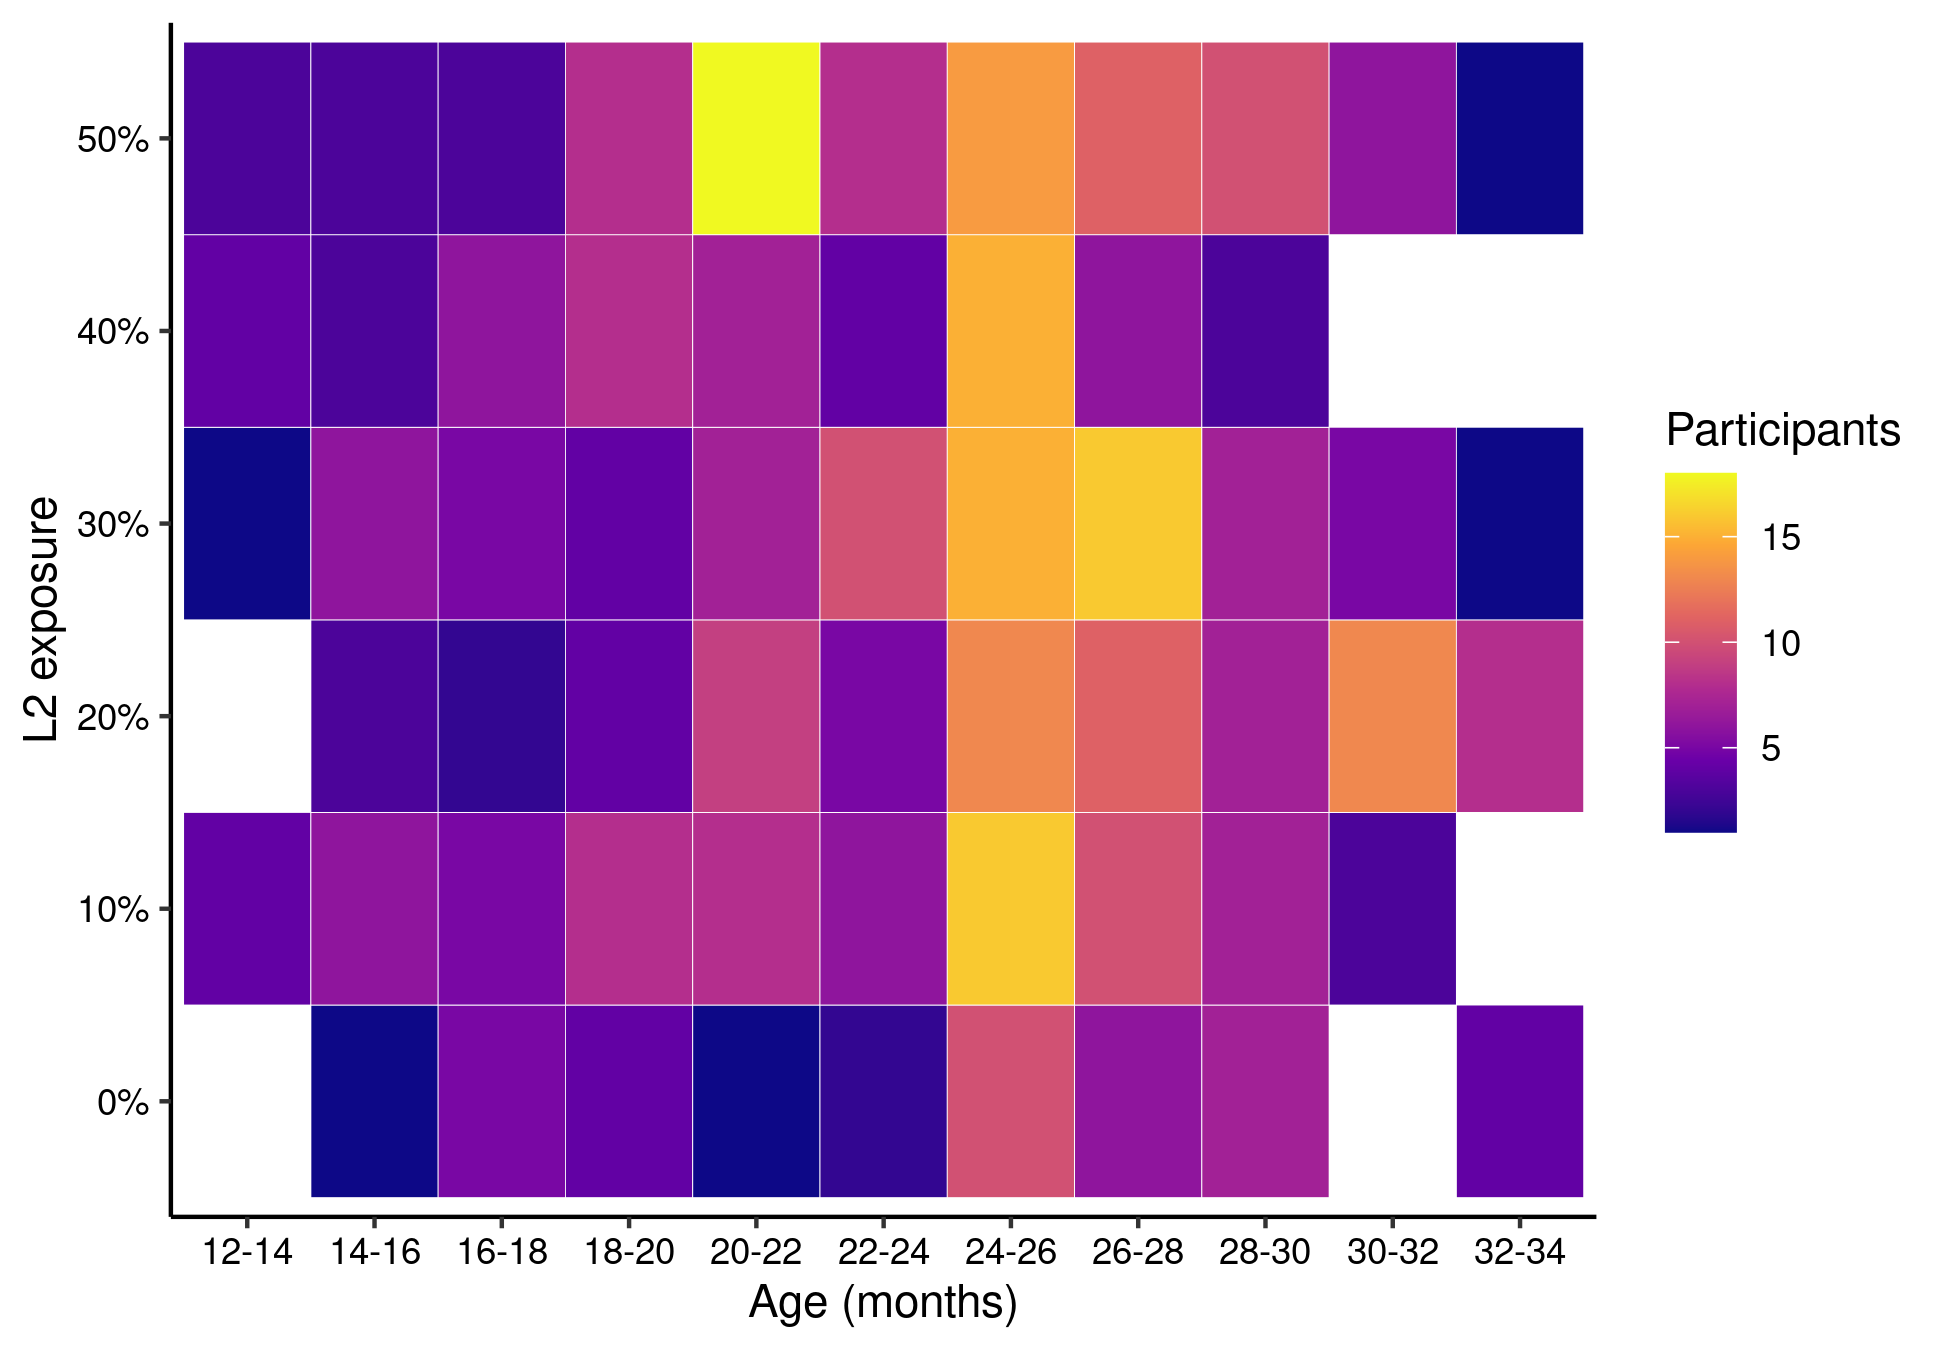
\includegraphics[width=0.8\linewidth]{trajectories_manuscript_files/figure-latex/lpdist-1} 

}

\caption{ }\label{fig:lpdist}
\end{figure}

\hypertarget{questionnaire}{%
\subsection{Questionnaire}\label{questionnaire}}

Parents completed an on-line questionnaire that gathered information about their demographic status, language environment of the child, and that included two vocabulary inventories: one for Catalan and one for Spanish. We implemented the questionnaire in \texttt{formr} (Arslan, Walther, \& Tata, 2020), a free, open-source platform. Participants were randomly allocated into one of four list of items. Each list contained a distinct inventory of translation equivalents. We included items from a diverse sample of 26 semantic/funcional categories: Action words, adventures, animals, body parts, clothes, color, descriptive words, food and drink, furniture and rooms, household items, on-line, outside, parts of animals, parts of things, people, pronouns, quantifiers, question words, time, toys, and vehicles. We discarded the following categories: adverbs, auxiliary words, connectives, interjections and games and routines. Those categories that did not entail more than 16 items - thus resulting in less than four items after dividing it in four lists - were not divided: all of their items were included in the four lists. Another subset of items that were part of the trial lsits of some experiments in the lab were also included in all versions.

Each item of the inventory presented a word-form, to which parents were instructed to report whether the toddlers was able to understand it, understand ans say it, or neither. The Catalan inventory contained 796 items (582 cognates, 195 non-cognates) and the Spanish inventory contained 801 (584 cognates, 197 non-cognates) . Items of one language were translation equivalents from the other (e.g., whenever \emph{gos} {[}dog{]} was included in the Catalan inventory, the word \emph{perro} was included in the Spanish inventory), roughly following a one-to-one mapping. When there were two acceptable translation equivalents for a given word, we included both (e.g., Catalan \emph{acabar} {[}\emph{to finish}{]} and Spanish \emph{acabar} and \emph{terminar}), or merged them into the same one (e.g., Spanish \emph{mono} {[}\emph{monkey}{]} and Catalan \emph{mono/mico}). We excluded from the analysis multi-word items (e.g., \emph{barrita de cereales} {[}cereal bar{]}) and items that included more than one word-form (e.g., \emph{mono / mico}).

\hypertarget{data-analysis}{%
\subsection{Data analysis}\label{data-analysis}}

For testing Hypothesis 1, we modelled the proportion of infants that understood or produced each item in the non-dominant language within age bins of 2 months. Our model assumes that this proportion follows a logistic curve across ages, an that the age of acquisition of each item is generated from a linear model that adjusts for the degree of exposure to the non-dominant language (\emph{bilingualism}, 0-50\%), the cognate status of the word (\emph{cognateness}, Non-cognate vs.~Cognate), and their interaction. Our prediction is that the age of acquisition will be lower for cognate words, compared to that of non-cognate words, and that this effect will be larger for more balanced bilinguals.

Items were classified into cognates and non-cognates by a trained Catalan-Spanish bilingual with broad experience in phonology and phonetics. Items were classified as L1 if the item was included in the inventory of the language the participant was dominant in, and as L2 if otherwise For instance, the item \emph{porta} (\emph{door}, in Catalan) was classified as L1 when answered by Catalan-dominant participants, and as L2 when answered by Spanish-dominant participants. Table \ref{tab:itemsinfo} shows the classification of items in cognates and non-cognates and their frequency scores across the four lists of the inventories.

\captionsetup[table]{labelformat=empty,skip=1pt}
\begin{longtable}{lcrrrrcrrrr}
\caption*{
\large \textbf{Questionnaire and item properties}\\ 
\small Participants were randomly allocated on of the the four lists, and completed both the Catalan and the Spanish versions.\\ 
} \\ 
\toprule
& \multicolumn{5}{c}{Frequency (Cognates)} & \multicolumn{5}{c}{Frequency (Non-cognates)} \\ 
 \cmidrule(lr){2-6}\cmidrule(lr){7-11}
\textbf{List} & \emph{N} & \emph{Mean} & \emph{SD} & \emph{Min} & \emph{Max} & \emph{N} & \emph{Mean} & \emph{SD} & \emph{Min} & \emph{Max} \\ 
\midrule
\multicolumn{1}{l}{Catalan} \\ 
\midrule
List A & $225$ & $4.47$ & $0.96$ & $1.25$ & $7.52$ & $100$ & $4.61$ & $1.06$ & $2.03$ & $7.44$ \\ 
List B & $227$ & $4.49$ & $0.90$ & $0.86$ & $7.52$ & $94$ & $4.40$ & $0.97$ & $1.94$ & $6.94$ \\ 
List C & $212$ & $4.46$ & $0.97$ & $1.67$ & $7.52$ & $106$ & $4.41$ & $1.00$ & $1.90$ & $6.94$ \\ 
List D & $212$ & $4.43$ & $0.85$ & $1.51$ & $7.52$ & $103$ & $4.45$ & $0.94$ & $2.10$ & $6.94$ \\ 
\midrule
\multicolumn{1}{l}{Spanish} \\ 
\midrule
List A & $222$ & $4.49$ & $0.99$ & $1.68$ & $7.12$ & $98$ & $4.47$ & $0.99$ & $2.28$ & $7.53$ \\ 
List B & $242$ & $4.35$ & $0.96$ & $1.68$ & $7.22$ & $95$ & $4.44$ & $0.93$ & $2.16$ & $7.53$ \\ 
List C & $228$ & $4.55$ & $1.02$ & $1.68$ & $7.52$ & $104$ & $4.58$ & $0.99$ & $2.87$ & $7.53$ \\ 
List D & $228$ & $4.41$ & $1.00$ & $1.68$ & $7.32$ & $106$ & $4.54$ & $1.05$ & $2.70$ & $7.53$ \\ 
\bottomrule
\end{longtable}

We fit two separate logistic models on comprehensive and productive data, respectively. Logistic curves are characterised by three parameters(see Mahr, 2019, and @mahr2020 for an excellent introduction to this approach, in which we based this analysis): (a) an \emph{asymptote} (\texttt{asym}, upper boundary of the proportion of infants that have acquired the item), (b) the \emph{steepness} (\texttt{steep}, how fast the a given item is acquired by infants), and (c) a \emph{mid-point} (\texttt{mid}, the age at which steepness is maximum). We work on the assumption that the trajectory of acquisition of items follows a logistic curve shape (Mayor \& Plunkett, 2011), and that the age of acquisition of a word is fairly captured by the position of the mid-point of its curve. This approach allows us to model and estimate the age of acquisition of items explicitly. Our model estimated the asymptote and steepness as grand means across items (i.e., intercepts). Mid-points were estimated by a linear regression model that included our predictors of interest: \texttt{age}, \texttt{item\_dominance} (sum-coded, L2 = -0.5, L1 = 0.5), \texttt{cognateness} (sum-coded, Non-cognate = -0.5, Cognate = 0.5). We also included random intercepts and \texttt{item\ dominance} slopes for each translation equivalent (\texttt{te}) ({\textbf{???}}). Appendix 1 shows a detailed description of the model.

We estimated the parameters of our model using the Bayesian framework. Bayesian models use the Bayes rule to combine prior knowledge about the distribution of a given parameter, and the likelihood of each of the values it can take given the data. We relied on the available data on Wordbank (Frank, Braginsky, Yurovsky, \& Marchman, 2017) to generate our priors (see Appendix 1 for more details about our prior). In order to test the contribution of each predictor on the fit of the model, we started fitting a null model that only included an global intercept and random intercepts for each TE, then fitted a model that also included \emph{bilingualism} and its random slopes by TE, and finally a model that also included \emph{cognateness} and its interaction with \emph{bilingualism}, as well as random slopes for all the fixed effects. We compared how the fit of the model changed in every step (Schad, Betancourt, \& Vasishth, 2020) using leave-one-out cross validation. We fit both the null and alternative models using the R environment (R Core Team, 2013; RStudio Team, 2015) and the \texttt{brms} package (Bürkner, 2017), which relies on the probabilistic language Stan (Carpenter et al., 2017) to approximate posterior distributions. We used Pareto-smoothed importance sampling (PSIS; Vehtari, Gelman, \& Gabry, 2017; Vehtari, Simpson, Gelman, Yao, \& Gabry, 2019) to compare the null and extended models. Data and model results were processed and visualised using the \texttt{tidyverse} family of R packages (Wickham et al., 2019) and the \texttt{tidybayes} package (Kay, 2020).

To test Hypothesis 2, we run a Bayesian ANOVA using the difference in mid-points between the two word-forms of each translation equivalent (in Catalan and Spanish, respectively), that included \emph{cognateness} as predictor. Using the \texttt{BayesFactor} R package (Morey \& Rouder, 2018), we computed a Bayes factor (\emph{BF}) that compared the likelihood of a linear model that included \emph{cognateness} as a predictor against the likelihood of a linear model that did not, under the light of our data.

\hypertarget{results}{%
\section{Results}\label{results}}

\hypertarget{hypothesis-1-are-cognates-acquired-ealier}{%
\subsection{Hypothesis 1: Are cognates acquired ealier?}\label{hypothesis-1-are-cognates-acquired-ealier}}

\hypertarget{comprehensive-data}{%
\paragraph{Comprehensive data}\label{comprehensive-data}}

\captionsetup[table]{labelformat=empty,skip=1pt}
\begin{longtable}{crrrrrl}
\toprule
Model & \emph{df} & AIC & BIC & Log. Likelihood & Likelihood ratio & \emph{p} \\ 
\midrule
$1$ & $5$ & $53,715.17$ & $53,761.83$ & $-26,852.58$ & - &  \\ 
$2$ & $6$ & $53,716.39$ & $53,772.38$ & $-26,852.20$ & $0.78$ & .378 \\ 
$3$ & $9$ & $51,646.15$ & $51,730.14$ & $-25,814.08$ & $2,076.24$ & < .001 \\ 
$4$ & $10$ & $51,702.84$ & $51,796.16$ & $-25,841.42$ & $54.69$ & < .001 \\ 
$5$ & $11$ & $51,565.73$ & $51,668.38$ & $-25,771.86$ & $139.11$ & < .001 \\ 
\bottomrule
\end{longtable}

\captionsetup[table]{labelformat=empty,skip=1pt}
\begin{longtable}{lcrrl}
\toprule
Term & Num. \emph{df} & Den. \emph{df} & \emph{F} & \emph{p} \\ 
\midrule
Asym & $1$ & $82,832.00$ & $60,748.66$ & < .001 \\ 
xmid.(Intercept) & $1$ & $82,832.00$ & $1,132.58$ & < .001 \\ 
xmid.frequency & $1$ & $82,832.00$ & $0.16$ & .693 \\ 
xmid.item\_dominance & $1$ & $82,832.00$ & $843.09$ & < .001 \\ 
xmid.cognate & $1$ & $82,832.00$ & $3.00$ & .083 \\ 
xmid.item\_dominance:cognate & $1$ & $82,832.00$ & $50.68$ & < .001 \\ 
scal & $1$ & $82,832.00$ & $7,635.78$ & < .001 \\ 
\bottomrule
\end{longtable}

\begin{figure}

{\centering 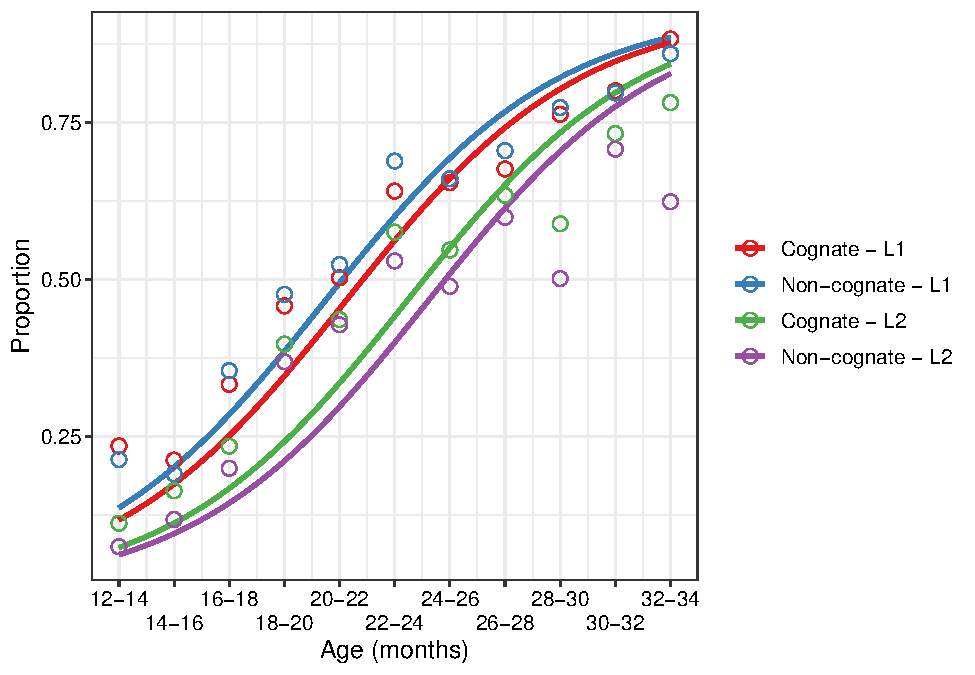
\includegraphics[width=0.8\linewidth]{trajectories_manuscript_files/figure-latex/comppredictions-1} 

}

\caption{ }\label{fig:comppredictions}
\end{figure}

\hypertarget{productive-data}{%
\subsubsection{Productive data}\label{productive-data}}

\captionsetup[table]{labelformat=empty,skip=1pt}
\begin{longtable}{crrrrrl}
\toprule
Model & \emph{df} & AIC & BIC & Log. Likelihood & Likelihood ratio & \emph{p} \\ 
\midrule
$1$ & $5$ & $23,516.51$ & $23,562.84$ & $-11,753.26$ & - &  \\ 
$2$ & $6$ & $23,503.04$ & $23,558.64$ & $-11,745.52$ & $15.47$ & < .001 \\ 
$3$ & $9$ & $21,344.08$ & $21,427.48$ & $-10,663.04$ & $2,164.96$ & < .001 \\ 
$4$ & $9$ & $21,343.35$ & $21,426.74$ & $-10,662.67$ & - &  \\ 
$5$ & $11$ & $21,291.22$ & $21,393.15$ & $-10,634.61$ & $56.13$ & < .001 \\ 
\bottomrule
\end{longtable}

\captionsetup[table]{labelformat=empty,skip=1pt}
\begin{longtable}{lcrrl}
\toprule
Term & Num. \emph{df} & Den. \emph{df} & \emph{F} & \emph{p} \\ 
\midrule
Asym & $1$ & $77,537.00$ & $5,719.12$ & < .001 \\ 
xmid.(Intercept) & $1$ & $77,537.00$ & $3,585.35$ & < .001 \\ 
xmid.frequency & $1$ & $77,537.00$ & $8.17$ & .004 \\ 
xmid.item\_dominance & $1$ & $77,537.00$ & $655.13$ & < .001 \\ 
xmid.cognate & $1$ & $77,537.00$ & $0.52$ & .473 \\ 
xmid.item\_dominance:cognate & $1$ & $77,537.00$ & $36.83$ & < .001 \\ 
scal & $1$ & $77,537.00$ & $4,870.09$ & < .001 \\ 
\bottomrule
\end{longtable}

\begin{figure}

{\centering 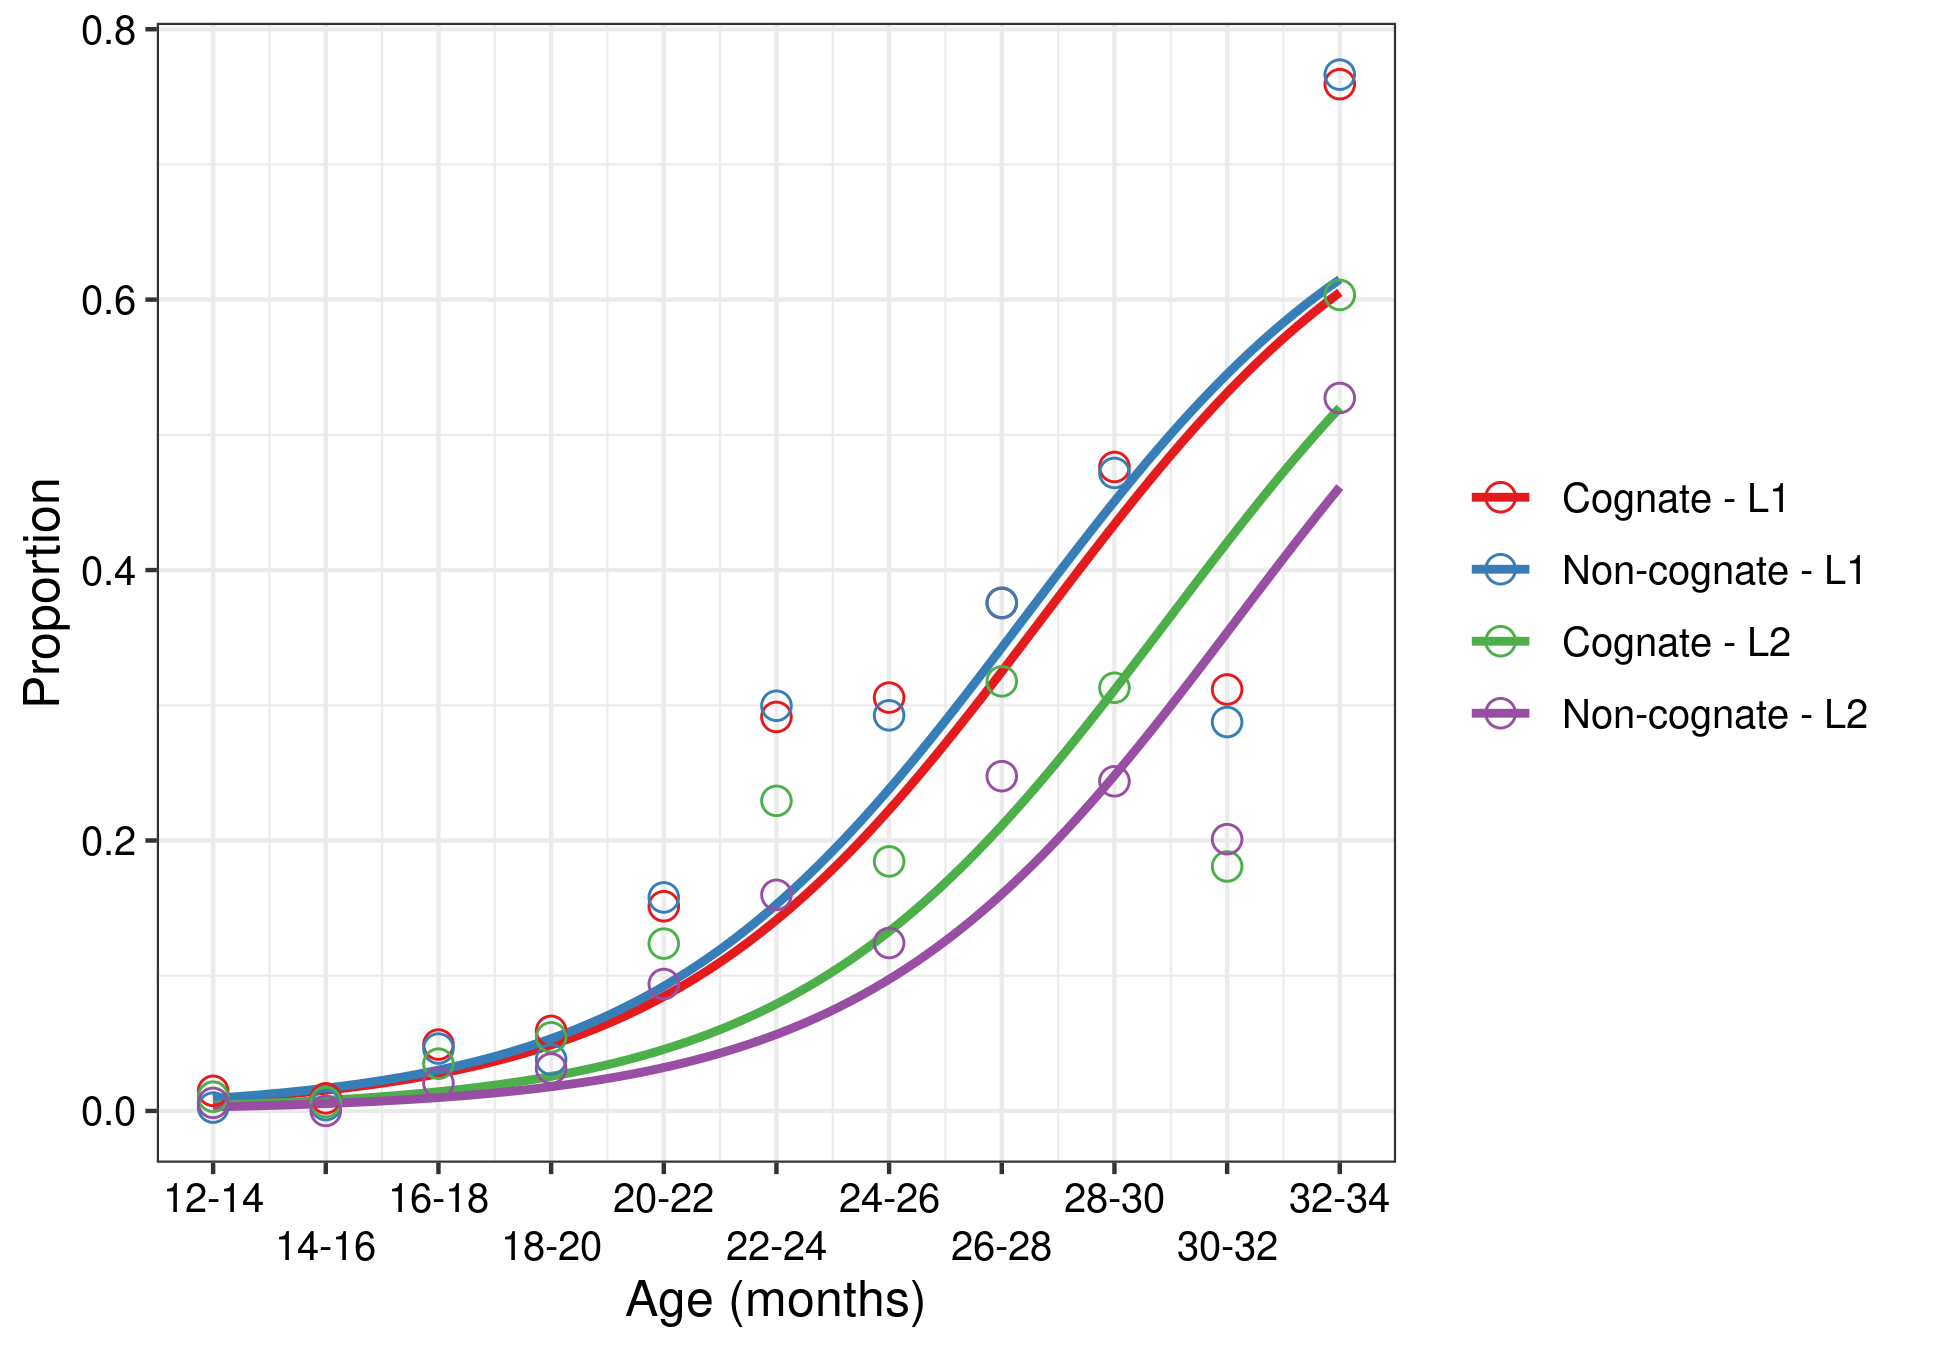
\includegraphics[width=0.8\linewidth]{trajectories_manuscript_files/figure-latex/prodpredictions-1} 

}

\caption{ }\label{fig:prodpredictions}
\end{figure}

\begin{figure}

{\centering 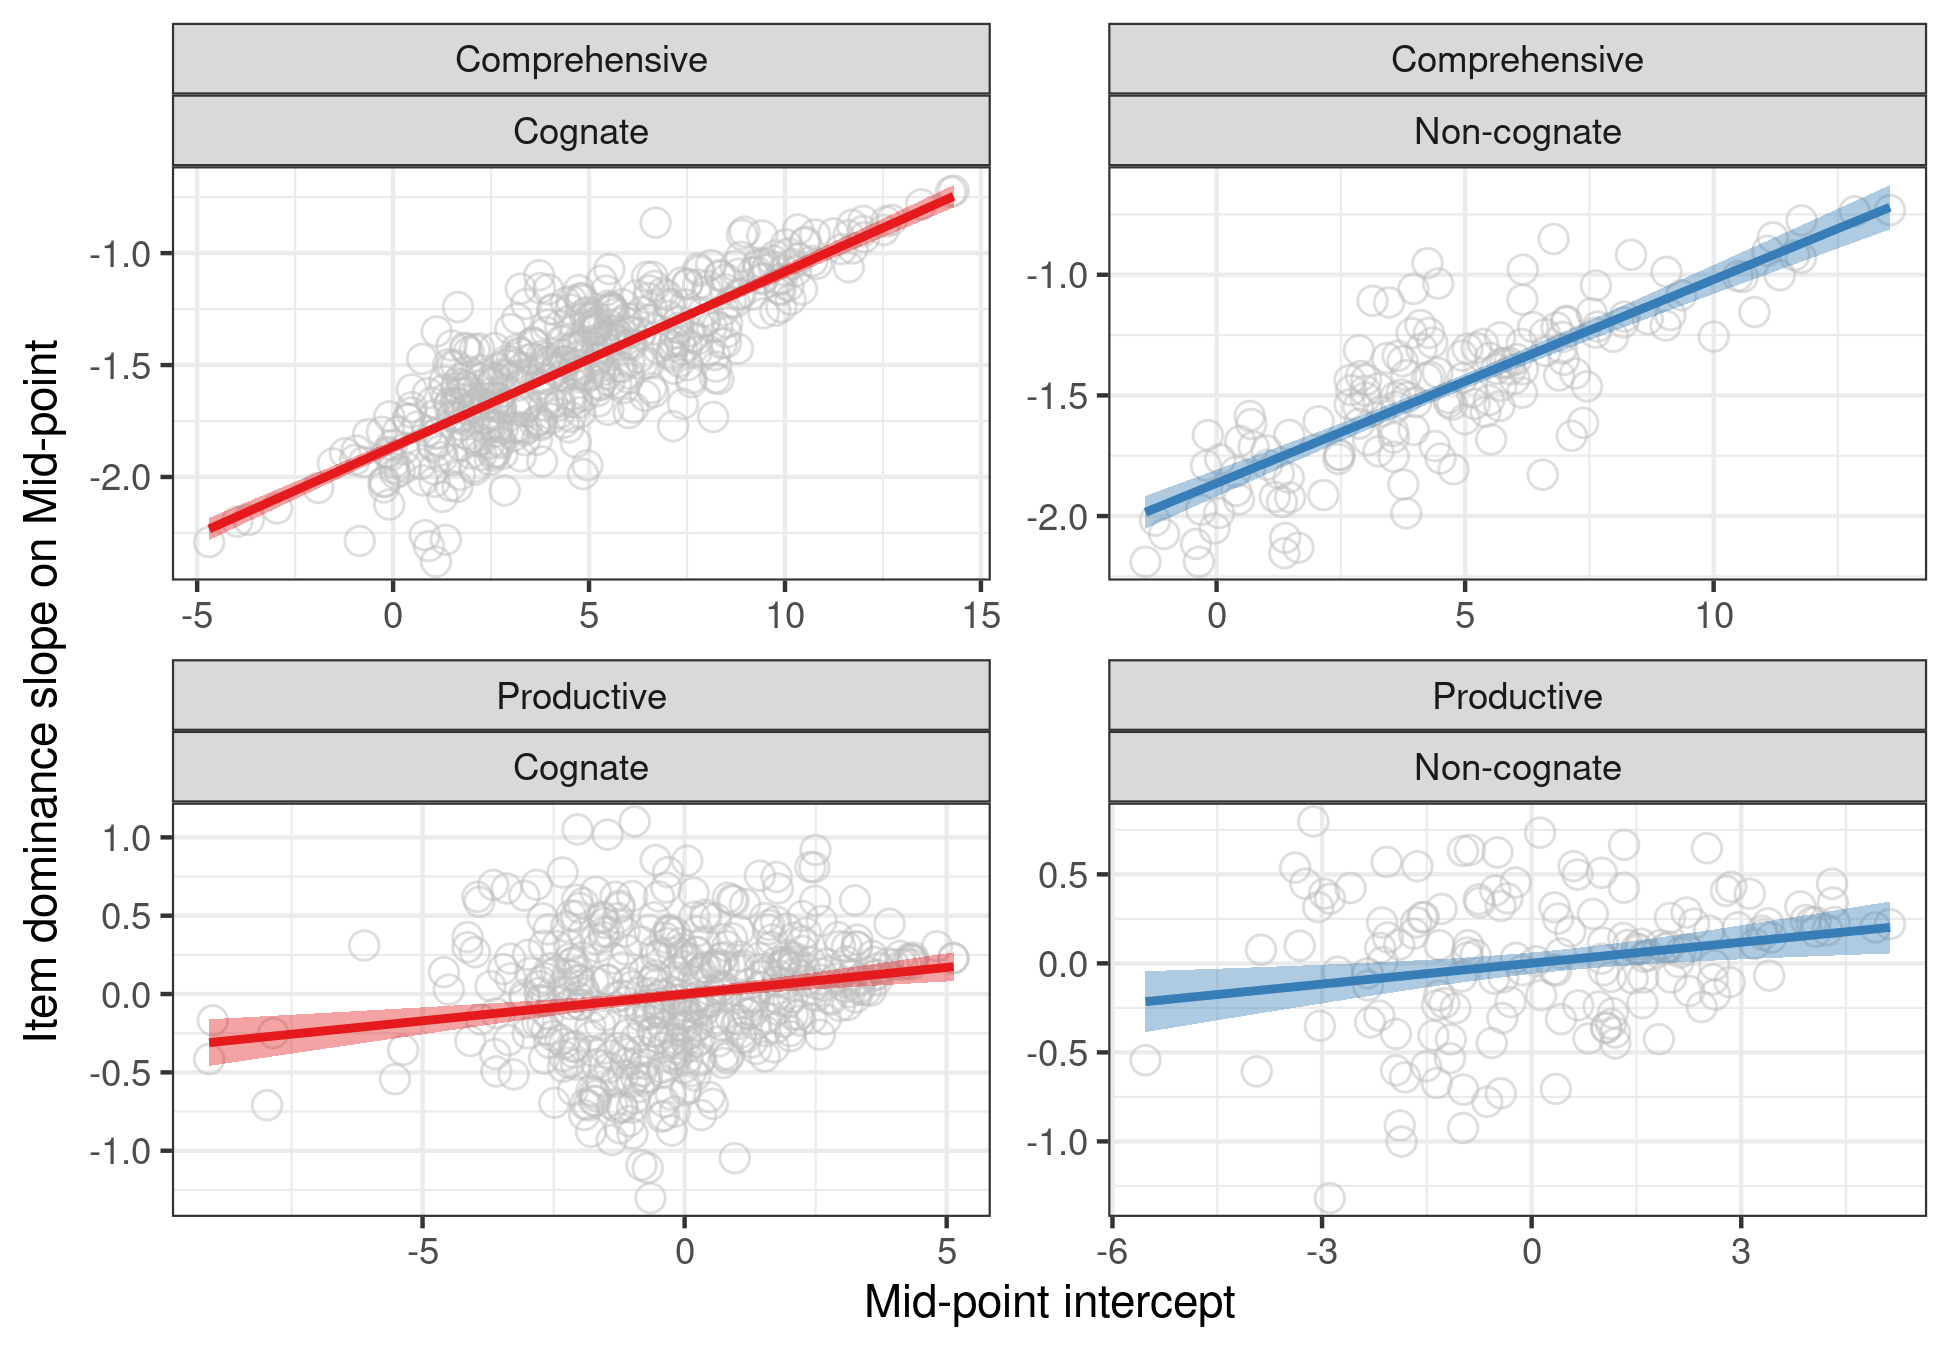
\includegraphics[width=0.8\linewidth]{trajectories_manuscript_files/figure-latex/ranefs-1} 

}

\caption{ }\label{fig:ranefs}
\end{figure}

\hypertarget{hypothesis-2}{%
\subsection{Hypothesis 2}\label{hypothesis-2}}

\begin{verbatim}
## Saving 6.5 x 4.5 in image
\end{verbatim}

\begin{figure}

{\centering 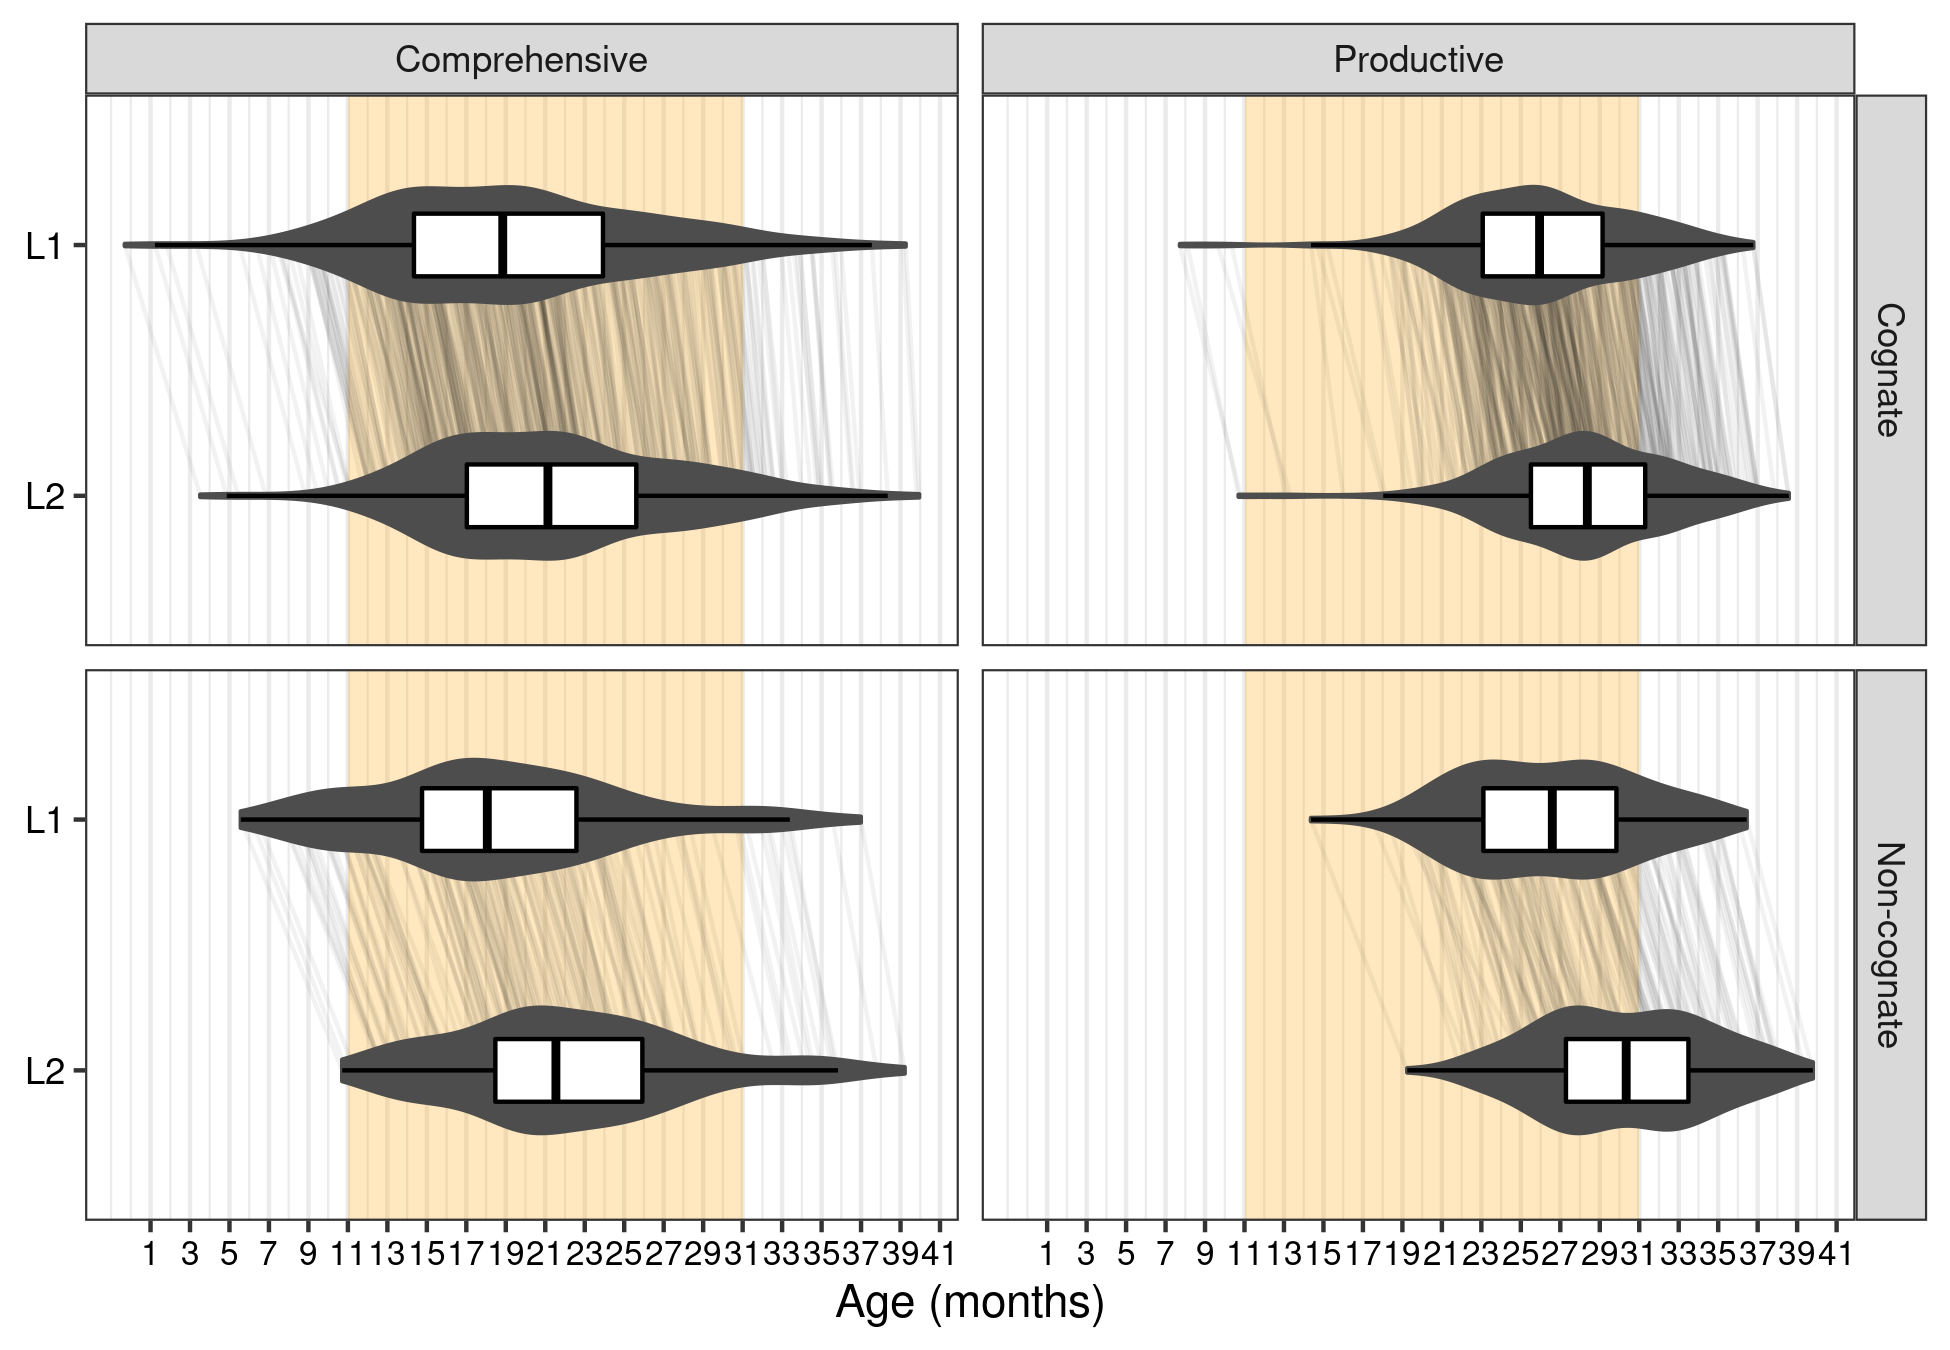
\includegraphics[width=0.8\linewidth]{trajectories_manuscript_files/figure-latex/aoafig-1} 

}

\caption{ }\label{fig:aoafig}
\end{figure}

\hypertarget{discussion}{%
\section{Discussion}\label{discussion}}

\hypertarget{appendix}{%
\section{Appendix}\label{appendix}}

\hypertarget{appendix-1-questionnaires}{%
\subsection{Appendix 1: Questionnaires}\label{appendix-1-questionnaires}}

\hypertarget{appendix-2-model-details}{%
\subsection{Appendix 2: Model details}\label{appendix-2-model-details}}

\hypertarget{appendix-3-session-info}{%
\subsection{Appendix 3: Session info}\label{appendix-3-session-info}}

R version 3.6.3 (2020-02-29)
Platform: x86\_64-pc-linux-gnu (64-bit)
Running under: Ubuntu 20.04.1 LTS

Matrix products: default
BLAS: /usr/lib/x86\_64-linux-gnu/blas/libblas.so.3.9.0
LAPACK: /usr/lib/x86\_64-linux-gnu/lapack/liblapack.so.3.9.0

locale:
{[}1{]} LC\_CTYPE=en\_GB.UTF-8 LC\_NUMERIC=C\\
{[}3{]} LC\_TIME=es\_ES.UTF-8 LC\_COLLATE=en\_GB.UTF-8\\
{[}5{]} LC\_MONETARY=es\_ES.UTF-8 LC\_MESSAGES=en\_GB.UTF-8\\
{[}7{]} LC\_PAPER=es\_ES.UTF-8 LC\_NAME=C\\
{[}9{]} LC\_ADDRESS=C LC\_TELEPHONE=C\\
{[}11{]} LC\_MEASUREMENT=es\_ES.UTF-8 LC\_IDENTIFICATION=C

attached base packages:
{[}1{]} stats graphics grDevices utils datasets methods base

other attached packages:
{[}1{]} rlang\_0.4.7 ggdist\_2.2.0 here\_0.1 data.table\_1.13.0
{[}5{]} gt\_0.2.1 modelr\_0.1.8 broom.mixed\_0.2.6 nlme\_3.1-145\\
{[}9{]} janitor\_2.0.1 lubridate\_1.7.9 readxl\_1.3.1 forcats\_0.5.0\\
{[}13{]} ggplot2\_3.3.2 tibble\_3.0.3 tidyr\_1.1.0 dplyr\_1.0.1\\
{[}17{]} magrittr\_1.5 knitr\_1.29 papaja\_0.1.0.9997

loaded via a namespace (and not attached):
{[}1{]} tidyselect\_1.1.0 xfun\_0.16 TMB\_1.7.18\\
{[}4{]} purrr\_0.3.4 reshape2\_1.4.4 splines\_3.6.3\\
{[}7{]} lattice\_0.20-40 snakecase\_0.11.0 colorspace\_1.4-1\\
{[}10{]} vctrs\_0.3.2 generics\_0.0.2 viridisLite\_0.3.0\\
{[}13{]} htmltools\_0.5.0 mgcv\_1.8-31 yaml\_2.2.1\\
{[}16{]} pillar\_1.4.6 glue\_1.4.1 withr\_2.2.0\\
{[}19{]} RColorBrewer\_1.1-2 distributional\_0.1.0 lifecycle\_0.2.0\\
{[}22{]} plyr\_1.8.6 stringr\_1.4.0 commonmark\_1.7\\
{[}25{]} munsell\_0.5.0 gtable\_0.3.0 cellranger\_1.1.0\\
{[}28{]} codetools\_0.2-16 coda\_0.19-3 evaluate\_0.14\\
{[}31{]} labeling\_0.3 fansi\_0.4.1 broom\_0.7.0.9001\\
{[}34{]} Rcpp\_1.0.5 checkmate\_2.0.0 scales\_1.1.1\\
{[}37{]} backports\_1.1.8 farver\_2.0.3 digest\_0.6.25\\
{[}40{]} stringi\_1.4.6 bookdown\_0.20 grid\_3.6.3\\
{[}43{]} rprojroot\_1.3-2 cli\_2.0.2 tools\_3.6.3\\
{[}46{]} crayon\_1.3.4 pkgconfig\_2.0.3 ellipsis\_0.3.1\\
{[}49{]} Matrix\_1.2-18 assertthat\_0.2.1 rmarkdown\_2.3\\
{[}52{]} R6\_2.4.1 compiler\_3.6.3

\hypertarget{references}{%
\section{References}\label{references}}

\begingroup
\setlength{\parindent}{-0.5in}
\setlength{\leftskip}{0.5in}

\hypertarget{refs}{}
\leavevmode\hypertarget{ref-arslan2020}{}%
Arslan, R. C., Walther, M. P., \& Tata, C. S. (2020). Formr: A study framework allowing for automated feedback generation and complex longitudinal experience-sampling studies using R. \emph{Behavior Research Methods}, \emph{52}(1), 376--387. \url{https://doi.org/10.3758/s13428-019-01236-y}

\leavevmode\hypertarget{ref-ben-zeev1977}{}%
Ben-Zeev, S. (1977). The Influence of Bilingualism on Cognitive Strategy and Cognitive Development. \emph{Child Development}, \emph{48}(3), 1009--1018. \url{https://doi.org/10.2307/1128353}

\leavevmode\hypertarget{ref-bialystok2010}{}%
Bialystok, E., Luk, G., Peets, K. F., \& Yang, S. (2010). Receptive vocabulary differences in monolingual and bilingual children. \emph{Bilingualism: Language and Cognition}, \emph{13}(4), 525--531. \url{https://doi.org/10.1017/S1366728909990423}

\leavevmode\hypertarget{ref-blom2019}{}%
Blom, E., Boerma, T., Bosma, E., Cornips, L., Heuij, K. van den, \& Timmermeister, M. (2019). Cross-language distance influences receptive vocabulary outcomes of bilingual children. \emph{First Language}, 0142723719892794. \url{https://doi.org/10.1177/0142723719892794}

\leavevmode\hypertarget{ref-bobb2020}{}%
Bobb, S. C., Von Holzen, K., Mayor, J., Mani, N., \& Carreiras, M. (2020). Co-activation of the L2 during L1 auditory processing: An ERP cross-modal priming study. \emph{Brain and Language}, \emph{203}, 104739. \url{https://doi.org/10.1016/j.bandl.2019.104739}

\leavevmode\hypertarget{ref-bosch2014}{}%
Bosch, L., \& Ramon-Casas, M. (2014). First translation equivalents in bilingual toddlers' expressive vocabulary: Does form similarity matter? \emph{International Journal of Behavioral Development}, \emph{38}(4), 317--322. \url{https://doi.org/10.1177/0165025414532559}

\leavevmode\hypertarget{ref-braginsky2019}{}%
Braginsky, M., Yurovsky, D., Marchman, V. A., \& Frank, M. C. (2019). Consistency and Variability in Children's Word Learning Across Languages. \emph{Open Mind}, \emph{3}, 52--67. \url{https://doi.org/10.1162/opmi_a_00026}

\leavevmode\hypertarget{ref-burkner2017}{}%
Bürkner, P.-C. (2017). Brms: An R Package for Bayesian Multilevel Models Using Stan. \emph{Journal of Statistical Software}, \emph{80}(1), 1--28. \url{https://doi.org/10.18637/jss.v080.i01}

\leavevmode\hypertarget{ref-carpenter2017}{}%
Carpenter, B., Gelman, A., Hoffman, M. D., Lee, D., Goodrich, B., Betancourt, M., \ldots{} Riddell, A. (2017). Stan: A Probabilistic Programming Language. \emph{Journal of Statistical Software}, \emph{76}(1), 1--32. \url{https://doi.org/10.18637/jss.v076.i01}

\leavevmode\hypertarget{ref-core2013}{}%
Core, C., Hoff, E., Rumiche, R., \& Señor, M. (2013). Total and Conceptual Vocabulary in Spanish--English Bilinguals From 22 to 30 Months: Implications for Assessment. \emph{Journal of Speech, Language, and Hearing Research}, \emph{56}(5), 1637--1649. \url{https://doi.org/10.1044/1092-4388(2013/11-0044)}

\leavevmode\hypertarget{ref-costa2000}{}%
Costa, A., Caramazza, A., \& Sebastian-Galles, N. (2000). The Cognate Facilitation Effect: Implications for Models of Lexical Access. \emph{Journal of Experimental Psychology}, \emph{26}(5), 1283--1296. \url{https://doi.org/10.1037/0278-7393.26.5.1283}

\leavevmode\hypertarget{ref-de1991lexical}{}%
De Groot, A. M., \& Nas, G. L. (1991). Lexical representation of cognates and noncognates in compound bilinguals. \emph{Journal of Memory and Language}, \emph{30}(1), 90--123.

\leavevmode\hypertarget{ref-dijkstra2002architecture}{}%
Dijkstra, A., \& Van Heuven, W. J. (2002). The architecture of the bilingual word recognition system: From identification to decision.

\leavevmode\hypertarget{ref-dijkstra2005}{}%
Dijkstra, T. (2005). Bilingual Visual Word Recognition and Lexical Access. In \emph{Handbook of bilingualism: Psycholinguistic approaches} (pp. 179--201). New York, NY, US: Oxford University Press.

\leavevmode\hypertarget{ref-dijkstra1998bia}{}%
Dijkstra, T., \& Van Heuven, W. J. (1998). The BIA model and bilingual word recognition. \emph{Localist Connectionist Approaches to Human Cognition}, 189--225.

\leavevmode\hypertarget{ref-dijkstra2019}{}%
Dijkstra, T., Wahl, A., Buytenhuijs, F., Halem, N. V., Al-Jibouri, Z., Korte, M. D., \& Rekké, S. (2019). Multilink: A computational model for bilingual word recognition and word translation. \emph{Bilingualism: Language and Cognition}, \emph{22}(4), 657--679. \url{https://doi.org/10.1017/S1366728918000287}

\leavevmode\hypertarget{ref-doyle1977some}{}%
Doyle, A. B., \& others. (1977). Some issues in the assessment of linguistic consequences of early bilingualism. \emph{Working Papers on Bilingualism}, (14).

\leavevmode\hypertarget{ref-fernandez1992}{}%
Fernandez, M. C., Pearson, B. Z., Umbel, V. M., Oiler, D. K., \& Molinet-Molina, M. (1992). Bilingual Receptive Vocabulary in Hispanic Preschool Children. \emph{Hispanic Journal of Behavioral Sciences}, \emph{14}(2), 268--276. \url{https://doi.org/10.1177/07399863920142006}

\leavevmode\hypertarget{ref-floccia2018}{}%
Floccia, C., Sambrook, T. D., Luche, C. D., Kwok, R., Goslin, J., White, L., \ldots{} Plunkett, K. (2018). I: Introduction. \emph{Monographs of the Society for Research in Child Development}, \emph{83}(1), 7--29. \url{https://doi.org/10.1111/mono.12348}

\leavevmode\hypertarget{ref-frank2017}{}%
Frank, M. C., Braginsky, M., Yurovsky, D., \& Marchman, V. A. (2017). Wordbank: An open repository for developmental vocabulary data. \emph{Journal of Child Language}, \emph{44}(3), 677--694. \url{https://doi.org/10.1017/S0305000916000209}

\leavevmode\hypertarget{ref-hoff2012}{}%
Hoff, E., Core, C., Place, S., Rumiche, R., Señor, M., \& Parra, M. (2012). Dual language exposure and early bilingual development*. \emph{Journal of Child Language}, \emph{39}(1), 1--27. \url{https://doi.org/10.1017/S0305000910000759}

\leavevmode\hypertarget{ref-hoff2014}{}%
Hoff, E., Rumiche, R., Burridge, A., Ribot, K. M., \& Welsh, S. N. (2014). Expressive vocabulary development in children from bilingual and monolingual homes: A longitudinal study from two to four years. \emph{Early Childhood Research Quarterly}, \emph{29}(4), 433--444. \url{https://doi.org/10.1016/j.ecresq.2014.04.012}

\leavevmode\hypertarget{ref-hoshino2008}{}%
Hoshino, N., \& Kroll, J. F. (2008). Cognate effects in picture naming: Does cross-language activation survive a change of script? \emph{Cognition}, \emph{106}(1), 501--511. \url{https://doi.org/10.1016/j.cognition.2007.02.001}

\leavevmode\hypertarget{ref-houwer2014}{}%
Houwer, A. D., Bornstein, M. H., \& Putnick, D. L. (2014). A bilingual--monolingual comparison of young children's vocabulary size: Evidence from comprehension and production. \emph{Applied Psycholinguistics}, \emph{35}(6), 1189--1211. \url{https://doi.org/10.1017/S0142716412000744}

\leavevmode\hypertarget{ref-kay2020}{}%
Kay, M. (2020). \emph{\textless span class="nocase"\textgreater tidybayes\textless/span\textgreater: Tidy data and geoms for Bayesian models} (manual). \url{https://doi.org/10.5281/zenodo.1308151}

\leavevmode\hypertarget{ref-kroll2013}{}%
Kroll, J. F., Gullifer, J. W., \& Rossi, E. (2013). The Multilingual Lexicon: The Cognitive and Neural Basis of Lexical Comprehension and Production in Two or More Languages. \emph{Annual Review of Applied Linguistics}, \emph{33}, 102--127. \url{https://doi.org/10.1017/S0267190513000111}

\leavevmode\hypertarget{ref-kroll2010}{}%
Kroll, J. F., Hell, J. G. V., Tokowicz, N., \& Green, D. W. (2010). The Revised Hierarchical Model: A critical review and assessment*. \emph{Bilingualism: Language and Cognition}, \emph{13}(3), 373--381. \url{https://doi.org/10.1017/S136672891000009X}

\leavevmode\hypertarget{ref-kroll1994}{}%
Kroll, J. F., \& Stewart, E. (1994). Category interference in translation and picture naming: Evidence for asymmetric connection between bilingual memory representations. \emph{Journal of Memory and Language}, \emph{33}(2), 149--174. \url{https://doi.org/10.1006/jmla.1994.1008}

\leavevmode\hypertarget{ref-mahr2019}{}%
Mahr, T. (2019). Anatomy of a logistic growth curve. \emph{Higher Order Functions}. Retrieved from \url{https://tjmahr.github.io/anatomy-of-a-logistic-growth-curve/}

\leavevmode\hypertarget{ref-mahr2020}{}%
Mahr, T. (2020). Bayes' theorem in three panels. \emph{Higher Order Functions}. Retrieved from \url{https://tjmahr.github.io/bayes-theorem-in-three-panels/}

\leavevmode\hypertarget{ref-mayor2011}{}%
Mayor, J., \& Plunkett, K. (2011). A statistical estimate of infant and toddler vocabulary size from CDI analysis. \emph{Developmental Science}, \emph{14}(4), 769--785. \url{https://doi.org/10.1111/j.1467-7687.2010.01024.x}

\leavevmode\hypertarget{ref-morey2018a}{}%
Morey, R. D., \& Rouder, J. N. (2018). \emph{BayesFactor: Computation of bayes factors for common designs} (manual). Retrieved from \url{https://CRAN.R-project.org/package=BayesFactor}

\leavevmode\hypertarget{ref-pearson1994}{}%
Pearson, B. Z., \& Fernández, S. C. (1994). Patterns of Interaction in the Lexical Growth in Two Languages of Bilingual Infants and Toddlers. \emph{Language Learning}, \emph{44}(4), 617--653. \url{https://doi.org/10.1111/j.1467-1770.1994.tb00633.x}

\leavevmode\hypertarget{ref-pearson1993}{}%
Pearson, B. Z., Fernández, S. C., \& Oller, D. K. (1993). Lexical Development in Bilingual Infants and Toddlers: Comparison to Monolingual Norms. \emph{Language Learning}, \emph{43}(1), 93--120. \url{https://doi.org/10.1111/j.1467-1770.1993.tb00174.x}

\leavevmode\hypertarget{ref-rcoreteam2013}{}%
R Core Team. (2013). \emph{R: A Language and Environment for Statistical Computing}. Vienna, Austria: R Foundation for Statistical Computing. Retrieved from \url{http://www.R-project.org/}

\leavevmode\hypertarget{ref-rosenblum1983word}{}%
Rosenblum, T., \& Pinker, S. A. (1983). Word magic revisited: Monolingual and bilingual children's understanding of the word-object relationship. \emph{Child Development}, 773--780. \url{https://doi.org/10.2307/1130064}

\leavevmode\hypertarget{ref-rstudioteam2015}{}%
RStudio Team. (2015). \emph{RStudio: Integrated Development Environment for R}. Boston, MA: RStudio, Inc. Retrieved from \url{http://www.rstudio.com/}

\leavevmode\hypertarget{ref-schad2020}{}%
Schad, D. J., Betancourt, M., \& Vasishth, S. (2020). Toward a principled Bayesian workflow in cognitive science. \emph{arXiv:1904.12765 {[}Stat{]}}. Retrieved from \url{http://arxiv.org/abs/1904.12765}

\leavevmode\hypertarget{ref-shook2013}{}%
Shook, A., \& Marian, V. (2013). The Bilingual Language Interaction Network for Comprehension of Speech*. \emph{Bilingualism: Language and Cognition}, \emph{16}(2), 304--324. \url{https://doi.org/10.1017/S1366728912000466}

\leavevmode\hypertarget{ref-thierry2007}{}%
Thierry, G., \& Wu, Y. J. (2007). Brain potentials reveal unconscious translation during foreign-language comprehension. \emph{Proceedings of the National Academy of Sciences}, \emph{104}(30), 12530--12535. \url{https://doi.org/10.1073/pnas.0609927104}

\leavevmode\hypertarget{ref-vehtari2017}{}%
Vehtari, A., Gelman, A., \& Gabry, J. (2017). Practical Bayesian model evaluation using leave-one-out cross-validation and WAIC. \emph{Statistics and Computing}, \emph{27}(5), 1413--1432. \url{https://doi.org/10.1007/s11222-016-9696-4}

\leavevmode\hypertarget{ref-vehtari2019}{}%
Vehtari, A., Simpson, D., Gelman, A., Yao, Y., \& Gabry, J. (2019). Pareto Smoothed Importance Sampling. \emph{arXiv:1507.02646 {[}Stat{]}}. Retrieved from \url{http://arxiv.org/abs/1507.02646}

\leavevmode\hypertarget{ref-vonholzen2019}{}%
Von Holzen, K., Fennell, C. T., \& Mani, N. (2019). The impact of cross-language phonological overlap on bilingual and monolingual toddlers' word recognition. \emph{Bilingualism: Language and Cognition}, \emph{22}(3), 476--499. \url{https://doi.org/10.1017/S1366728918000597}

\leavevmode\hypertarget{ref-vonholzen2012}{}%
Von Holzen, K., \& Mani, N. (2012). Language nonselective lexical access in bilingual toddlers. \emph{Journal of Experimental Child Psychology}, \emph{113}(4), 569--586. \url{https://doi.org/10.1016/j.jecp.2012.08.001}

\leavevmode\hypertarget{ref-wickham2019}{}%
Wickham, H., Averick, M., Bryan, J., Chang, W., McGowan, L. D., François, R., \ldots{} Yutani, H. (2019). Welcome to the \textless span class="nocase"\textgreater tidyverse\textless/span\textgreater. \emph{Journal of Open Source Software}, \emph{4}(43), 1686. \url{https://doi.org/10.21105/joss.01686}

\leavevmode\hypertarget{ref-yudes2010}{}%
Yudes, C., Macizo, P., \& Bajo, T. (2010). Cognate effects in bilingual language comprehension tasks. \emph{NeuroReport}, \emph{21}(7), 507--512. \url{https://doi.org/10.1097/WNR.0b013e328338b9e1}

\endgroup


\end{document}
